\section{Background}
Technological advancement has revolutionized the field of genomics, which has led to a cost-effective generation of big amounts of sequence data. The sequencing of the first human genome (2002) took around 13 years and cost over \$3 million to complete. Nowadays we can resequence a human genome for \$1000 and can generate more than 320 genomes per week\cite{big_biological_impacts_bd}. This technological innovation leads to the accumulation of vast quantities of genomic data, posing a tremendous challenge to scientists for effective mining of data to explain a phenomenon of interest. New ways of analysing the produced data have been therefore necessary in order to discover interesting patterns  and make the most out of it. No matter how much resources we use into extracting the data if we don't get anything interesting out of it\cite{zhang_paciorkowski_craig_cui_2019}.

Some of the main problems that researchers face when analysing genomic data are information overload, data interconnectivity and high dimensionality. Visualization is one way of facing this problems. For this reason it is very important to implement efficient visualization technologies that can lead to find new patterns and the extraction of good conclusions of the data. In the field of system biology there are usually network representations where the nodes or bioentities are connected to each other, where these edges represent associations. Because of the improvements in technology, these networks can increase dramatically in size and complexity. We need therefore better visualization systems and more efficient alogirithms for the analysis of the data.

In \ref{fig:network_biology_evolution} we can see a representation of the evolution for visualization of networks in system biology. From simple graphs in 2 dimensions, to 3D representations and nowadays also visualizations in virtual reality where we can interact directly with the data itself.

\begin{figure}[h!]
    \newlength{\tempheight}
    \setlength{\tempheight}{15ex}
    \centering%
    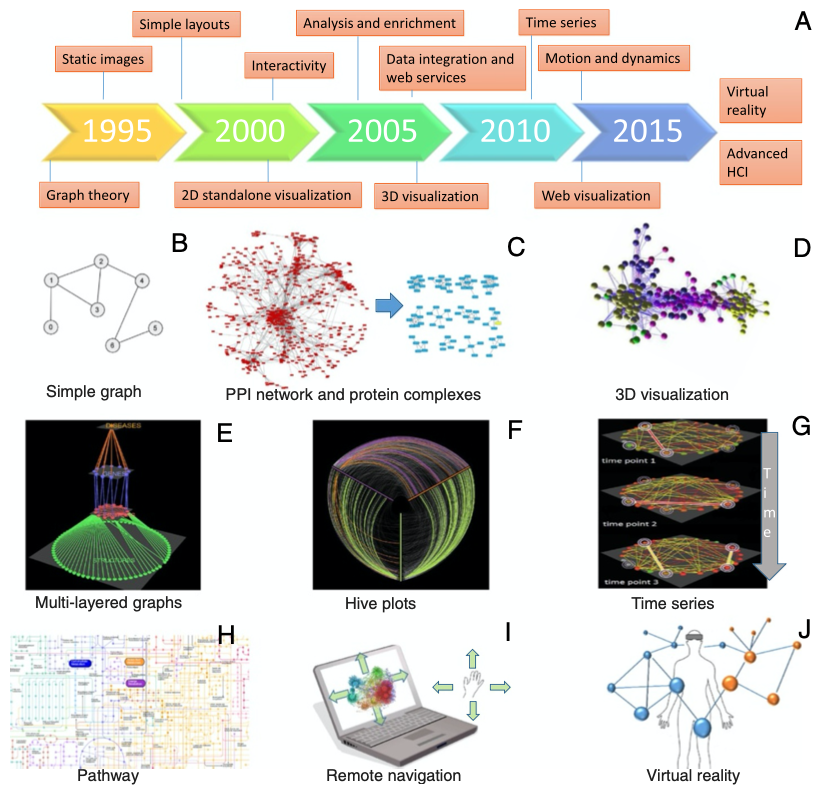
\includegraphics[width=\textwidth]{evolution_visualization}
    \caption{Visualization for network biology. a A simple drawing of an undirected unweighted graph. b A 2D representation of a yeast protein-protein interaction network visualized in Cytoscape (left) and potential protein complexes 3D identified by the MCL algorithm from that network (right). c A 3D view of a protein-protein interaction network visualized by BiolayoutExpress. d A multilayered network integrating different types of data visualized by Arena3D. e A hive plot view of a network in which nodes are mapped to and positioned on radially distributed linear axes. f Visualization of network changes over time. g Part of lung cancer pathway visualized by iPath. i Remote navigation and control of networks by hand gestures. h Integration and control of 3D networks using VR devices. Figure adapted\cite{pavlopoulos_malliarakis_papanikolaou_theodosiou_enright_iliopoulos_2015}.}
    \label{fig:network_biology_evolution}
\end{figure}%

Virtual reality (VR) is still a field under exploration and that can be of great help in network analysis. VR can be very powerful because it takes advantage of the way the human being perceives and analysis things. We as human beings have a great ability to discover patterns, however we are biologically optimized to see the world and the patterns in 3 dimensions. VR is one of the best ways then for better discovery in spatial dimensions. It has been demonstrated that VR help scientists work more effectively in fields like medicine \cite{Laver11}\cite{xia_ip_samman_wong_gateno_wang_yeung_kot_tideman_2001}\cite{brain_damage_rehab}, biology\cite{10.1093/bioinformatics/bti581}\cite{thorley_lawson_duca_shapiro_2008} and neuroscience\cite{bohil_alicea_biocca_2011}\cite{minderer_harvey_donato_moser_2016}, to cite some examples.


\section{Challenges and research problem}
This project focus mainly on solving the problem of visualization of high dimenasional data from the MIxT project by using virtual reality. Furthermore the application allows the user to interact with the network created from the data in the virtual environment. It also allows the user compare the blood and biopsy networks at the same time in order to finde relationship, which wasn't possible in the MIxT web application as this only allows the user to visualize one network at a time.

MIxT\cite{fjukstad_dumeaux_olsen_lund_hallett_bongo_2017} is a web application for bioinformaticians. Among other tools, it offers a network visualization of genes which are represented as nodes in the network and where the edges represent statistically significant correlation in expression between two nodes. This tool was used in a study\cite{dumeaux_fjukstad_interactions_tumor_blood} that identifies genes and pathways in the primary tumor that are tightly linked to genes and pathways in the systemic response of a patient with breast cancer.
When exploring a network in MIxT, it can be hard to understand the data and its relationships because there is too much data. This problem is easy to occur when there are too many node and edges. In figure \ref{fig:mixt_network} we can see an example of the network visualization from MIxT. As we can see in Figure \ref{fig:mixt_network1}, there are many nodes and relationships among them and when we zoom in in the network, it becomes very difficult to understand the data and the relationships as shown in in Figure \ref{fig:mixt_network_zoom}.

 The network is also in 2-dimensions and what we propose in this project is to use a virtual reality 3d visualization in order to cope better with this problem.

\begin{figure}[h!]
    \centering%
    \begin{subfigure}[t]{0.5\textwidth}
        \centering%
        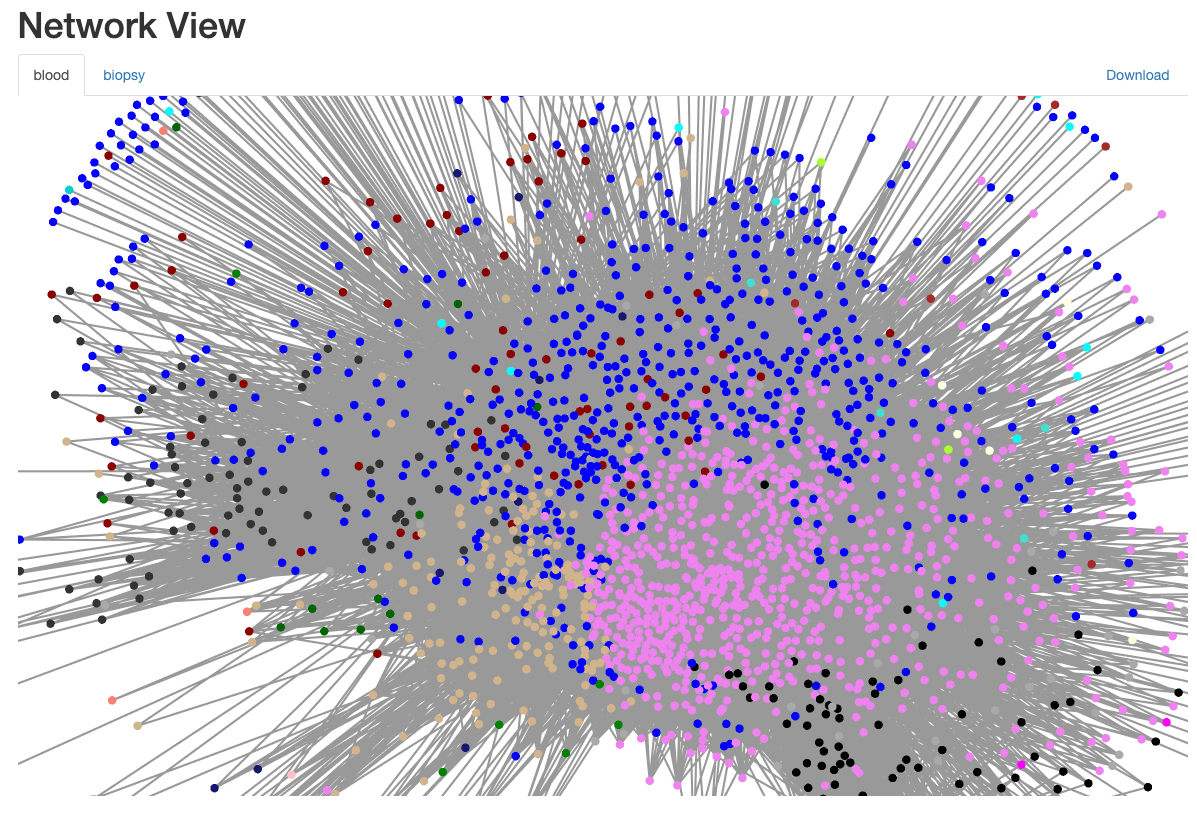
\includegraphics[width=\linewidth]{mixt_network1}
        \caption{Network with several modules.}
        \label{fig:mixt_network1}
    \end{subfigure}%
    \begin{subfigure}[t]{0.5\textwidth}
        \centering%
        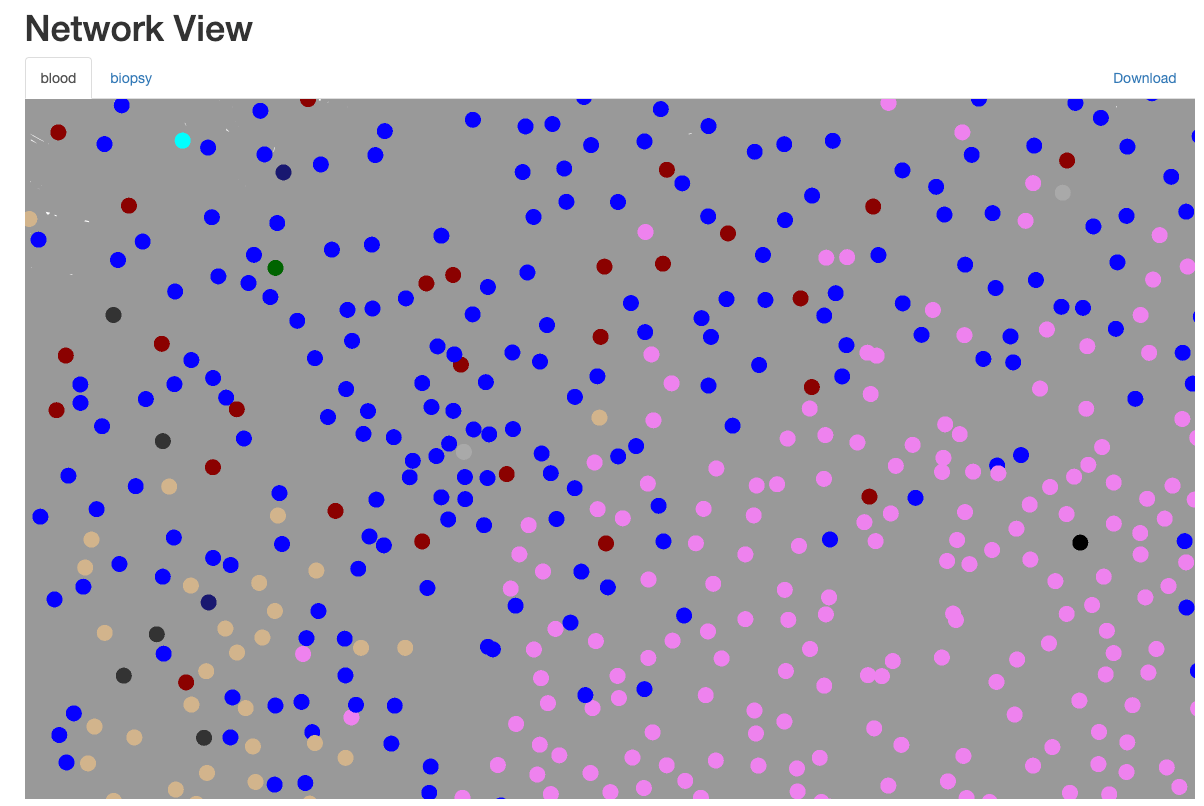
\includegraphics[width=\linewidth]{mixt_network2}
        \caption{Zoom in the network.}
        \label{fig:mixt_network_zoom}
    \end{subfigure}

    \caption{Network view of the MIxT application where nodes repsent genes and the modules are repsented by colors. Relationships are represented by grey lines that connect a gene with another one.}
    \label{fig:mixt_network}
\end{figure}

\section{Proposed solution}

\section{Significance and contribution}
This project contributes in the exploration of the possibilities that Virtual Reality offers for visualization of big data in bioinformatics.

\section{Outline}
